% =====================================================================
\section{Simulation design}
\label{sec:data}

Two synthetic datasets were generated with the procedure below (implementation in \texttt{gfer/demo.py}). They are designed so that every pipeline stage has something to find and, crucially, so that the windows carrying class information are known.

\paragraph{Structure.} Each dataset has 5 simulated subjects and 12 trials per subject (3 per class: sad, happy, fear, neutral), i.e.\ 60 trials of 60~s and 900 four-second windows. EEG has 62 channels in the SEED-IV montage at 200~Hz; eye tracking has 60~Hz pupil diameters in the horizontal and vertical directions and a fixation sequence.

\paragraph{Background EEG.} Eight pink-noise sources are mixed into the channels through a subject-specific random matrix, with posterior alpha activity, independent channel noise, 50~Hz line interference and channel DC offsets.

\paragraph{Emotional episodes.} Each trial contains three non-overlapping episodes of 6--10~s placed at random after the first 4~s (mean length 7.9~s in SIM-H and 8.1~s in SIM-E). On average 39.3\% (SIM-H) and 40.3\% (SIM-E) of windows overlap an episode by at least half their length. Class information exists in the EEG \emph{only} during episodes: a band-limited component with class-specific bandwidth, amplitude and burstiness (sad narrow-band and regular, happy medium bandwidth, fear broadband and bursty, neutral none) is added to T7, T8, Fp2 and neighbouring channels, with band strengths alpha $>$ beta $>$ gamma $>$ theta $>$ delta, and a subject-specific gain.

\paragraph{Eye-tracking signals.} During episodes the vertical pupil diameter dilates by a class-dependent amount (0.35--0.65~mm; the horizontal diameter by 60\% of this) with 1.5-s ramps, on top of a subject-specific baseline (3.0--4.2~mm) and a slow random drift. Two \emph{distractor} dilations of 3--5~s (0.25~mm) per trial carry no EEG change, so the pupil is an informative but imperfect indicator. About 15 blinks per trial are inserted as missing samples. Fixation durations are gamma-distributed around 260~ms and are multiplied by a class-dependent factor (sad 1.35, happy 1.10, fear 0.80, neutral 1.00) during episodes, so fixation features carry class information but only weak episode information.

\paragraph{Difficulty levels.} SIM-H (``harder'') uses class-signal strength 1.0 and generator seed 0; SIM-E (``easier'') uses strength 3.0 and seed 1. Both datasets were regenerated from these settings and verified to be identical to the files used in the experiments.

Table~\ref{tab:simdata} summarises the design. The simulation deliberately encodes the assumption that motivates gating, namely that affective information is intermittent and that pupil dilation co-occurs with it. The results therefore show how the gates behave when this assumption holds; they do not show that it holds in real recordings.

\begin{table}[t]
\centering\small
\caption{Synthetic datasets (generator \texttt{gfer/demo.py})}\label{tab:simdata}
\begin{tabular}{@{}lll@{}}
\toprule
Property & SIM-H & SIM-E\\
\midrule
Subjects / trials / windows & 5 / 60 / 900 & 5 / 60 / 900\\
Classes (trials per class) & sad, happy, fear, neutral (15 each) & same\\
EEG & 62 ch, 200 Hz, 60 s per trial & same\\
Eye tracking & pupil X/Y 60 Hz, fixations, blinks & same\\
Episodes per trial; windows in episode & 3; 39.3\% & 3; 40.3\%\\
Distractor pupil dilations per trial & 2 & 2\\
Class-signal strength; seed & 1.0; 0 & 3.0; 1\\
\bottomrule
\end{tabular}
\end{table}

% =====================================================================
\section{Experimental setup}
\label{sec:setup}

\paragraph{Configurations.} Four gates are compared: A1 (no gate), M0 (hard), M1 (fuzzy) and A4 (linear soft). Each is run with both gating-feature choices (G-pupil and G-mRMR), on both datasets, for all five bands, with three fuzzy levels per input.

\paragraph{Validation and leakage control.} Evaluation is at trial level. Two protocols are used: (P1) stratified trial-disjoint 5-fold CV, with 12 test trials per fold, and (P2) leave-one-subject-out (LOSO) CV over the 5 subjects. No trial (P1) or subject (P2) contributes windows to both training and test data. All label-dependent steps, namely gating-feature selection in G-mRMR, EEG mRMR, discretisation and the GA, are fitted on training trials only. The two label-free normalisations (per-subject z-scoring of entropies and per-trial scaling of the gating feature) are applied identically to every configuration. Each setting is repeated with three seeds, which change the P1 fold assignment and the GA's random operations, giving 15 (seed, band) results per configuration, dataset and protocol. M0, M1, A1 and A4 share folds and seeds.

\paragraph{Gate-noise robustness.} To test the claim that fuzzy gating tolerates an uncertain eye signal, Gaussian noise with standard deviation $\kappa\in\{0.5,1,2\}$ times the within-subject standard deviation of the pupil feature is added to the G-pupil gating feature before normalisation (protocol P1, all bands, three seeds).

\paragraph{Gate quality.} Because episodes are known, the gates are also assessed directly. For each window, the label ``in episode'' is compared with the normalised gating feature (AUC), with the hard gate's retained set (precision and recall) and with the soft gates' weights (weighted precision $\sum_k w_k e_k/\sum_k w_k$, where $e_k=1$ if window $k$ lies in an episode).

\paragraph{Metrics and statistics.} Accuracy, balanced accuracy and macro-averaged precision, recall and F1 are computed over the pooled trial predictions of all folds of a run. Because classes are balanced, balanced accuracy equals macro recall and chance accuracy is 25\%. M1 is compared with M0, A4 and A1 using the Wilcoxon signed-rank test over the 15 paired (seed, band) accuracies \cite{Demsar2006}. For the best band, an exact McNemar test \cite{McNemar1947} on paired trial predictions pooled over seeds is also reported; pooling over seeds makes the pairs non-independent, so this test is indicative only. No correction for multiple comparisons is applied in the tables, and the 24 M1 comparisons are interpreted with this in mind.

\paragraph{Implementation.} The pipeline is implemented in Python 3.13.7 with NumPy 2.5.4, SciPy 1.18.1, scikit-learn 1.9.1, PyWavelets 1.8.0 and Matplotlib 3.11.2. Experiments ran on an Apple M2 (8 cores, 8~GB RAM, macOS 26.5) with 8 worker processes. The main grids took 425~s (G-mRMR) and 303~s (G-pupil), and the noise sweep 773~s, using cached features. Code: \pending{repository URL}.

% =====================================================================
\section{Results and discussion}
\label{sec:results}

\noindent\emph{All results in this section are simulation results\simnote{} on SIM-H and SIM-E.}

\subsection{How well do the gating signals locate the episodes?}
Table~\ref{tab:gateq} measures each gate against the known episodes. The vertical pupil feature separates episode from non-episode windows almost perfectly (AUC 0.987 on SIM-H and 0.985 on SIM-E). The hard gate built on it retains windows of which 90.3\% (SIM-H) and 92.8\% (SIM-E) lie in episodes, against base rates of 39.3\% and 40.3\%, while recovering 91.8\% and 92.0\% of episode windows. The fuzzy gate places a mean weight of 0.84 on episode windows and 0.15 on the others, but because every window keeps a weight of at least $r_L=0.1$ and Medium-range windows receive about 0.5, its weighted precision is lower (78.7\% and 79.4\%); the linear gate is lower still (75.0\% and 75.8\%). Figure~\ref{fig:trace} shows both gates on one trial.

In G-mRMR, the label-driven selection never chose a pupil feature. Across all folds it chose the mean fixation duration (53\% of folds on SIM-H, 70\% on SIM-E) or the fixation frequency (the remainder). These features are class-discriminative by construction but are poor episode indicators: mean fixation duration has an episode AUC of only 0.576 and 0.566, and the hard gate built on it retains windows that are only 46.1\% and 50.0\% in-episode, barely above the base rates.

\begin{table}[t]
\centering\scriptsize
\caption{Gate quality against the known episodes\simnote{} (all 900 windows per dataset). w-prec.: weighted precision}\label{tab:gateq}
\begin{tabular}{@{}llccccc@{}}
\toprule
Data & Gate feature & Episode rate & AUC($\tilde z$) & Hard: prec./recall & Fuzzy: w-prec. & Linear: w-prec.\\
\midrule
SIM-H & \texttt{pupil\_y\_mean} & 39.3\% & 0.987 & 90.3\% / 91.8\% & 78.7\% & 75.0\%\\
SIM-H & \texttt{fix\_dur\_mean} & 39.3\% & 0.576 & 46.1\% / 46.9\% & 44.1\% & 43.4\%\\
SIM-E & \texttt{pupil\_y\_mean} & 40.3\% & 0.985 & 92.8\% / 92.0\% & 79.4\% & 75.8\%\\
SIM-E & \texttt{fix\_dur\_mean} & 40.3\% & 0.566 & 50.0\% / 49.6\% & 45.0\% & 44.3\%\\
\bottomrule
\end{tabular}

\end{table}

\begin{figure}[t]
\centering
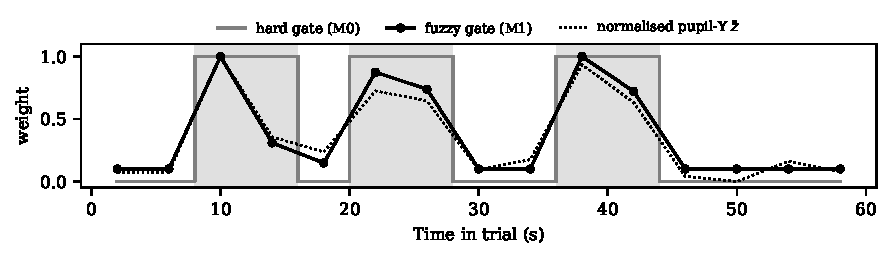
\includegraphics[width=0.85\linewidth]{generated/fig_gate_trace.pdf}
\caption{Hard and fuzzy gate weights on one synthetic trial (SIM-E, subject S01, trial T01) with the G-pupil feature\simnote. Shaded windows overlap a simulated episode.}
\label{fig:trace}
\end{figure}

\subsection{Overall comparison}
Table~\ref{tab:main} reports metrics averaged over bands and seeds for G-pupil. With an informative gating signal, gating of any form helped substantially. Under P1, mean accuracy rose from 35.8\% (A1) to 55.2\% (M0) and 54.9\% (M1) on SIM-H, and from 49.1\% to 66.0\% and 65.7\% on SIM-E. Macro-F1 followed the same pattern (SIM-H 32.8\%, 53.1\%, 52.1\%; SIM-E 45.8\%, 63.9\%, 62.8\%). LOSO gave similar values (SIM-H: 39.9\%, 52.6\%, 54.0\%; SIM-E: 47.4\%, 66.1\%, 65.9\%). The difference between M1 and M0 is at most 1.4~pp in either direction in all four dataset--protocol cells. The linear gate A4 was within 4.4~pp of both. The large standard deviations reflect differences between bands rather than between seeds (Sect.~\ref{sec:bands}).

\begin{table}[t]
\centering\scriptsize
\caption{Trial-level performance with the G-pupil gating feature\simnote{} (\%, mean $\pm$ SD over 5 bands $\times$ 3 seeds). Top: P1 trial-disjoint 5-fold CV; bottom: P2 LOSO}\label{tab:main}
\begin{tabular}{@{}llccccc@{}}
\toprule
Data & Configuration & Accuracy & Bal.\ acc. & Macro P & Macro R & Macro F1\\
\midrule
SIM-H & No gate (A1) & 35.8 $\pm$ 9.2 & 35.8 $\pm$ 9.2 & 39.1 $\pm$ 14.6 & 35.8 $\pm$ 9.2 & 32.8 $\pm$ 9.7\\
 & Hard gate, M0 & 55.2 $\pm$ 25.0 & 55.2 $\pm$ 25.0 & 55.9 $\pm$ 26.4 & 55.2 $\pm$ 25.0 & 53.1 $\pm$ 25.0\\
 & Fuzzy gate, M1 & 54.9 $\pm$ 20.7 & 54.9 $\pm$ 20.7 & 52.4 $\pm$ 20.4 & 54.9 $\pm$ 20.7 & 52.1 $\pm$ 20.6\\
 & Linear soft gate (A4) & 53.2 $\pm$ 18.3 & 53.2 $\pm$ 18.3 & 52.4 $\pm$ 17.3 & 53.2 $\pm$ 18.3 & 50.6 $\pm$ 16.9\\
\midrule
SIM-E & No gate (A1) & 49.1 $\pm$ 8.4 & 49.1 $\pm$ 8.4 & 52.0 $\pm$ 12.6 & 49.1 $\pm$ 8.4 & 45.8 $\pm$ 7.4\\
 & Hard gate, M0 & 66.0 $\pm$ 21.3 & 66.0 $\pm$ 21.3 & 66.3 $\pm$ 24.2 & 66.0 $\pm$ 21.3 & 63.9 $\pm$ 22.7\\
 & Fuzzy gate, M1 & 65.7 $\pm$ 21.1 & 65.7 $\pm$ 21.1 & 65.3 $\pm$ 24.1 & 65.7 $\pm$ 21.1 & 62.8 $\pm$ 22.1\\
 & Linear soft gate (A4) & 64.8 $\pm$ 15.2 & 64.8 $\pm$ 15.2 & 65.0 $\pm$ 20.2 & 64.8 $\pm$ 15.2 & 61.0 $\pm$ 16.0\\
\bottomrule
\end{tabular}
\\[4pt]
\begin{tabular}{@{}llccccc@{}}
\toprule
Data & Configuration & Accuracy & Bal.\ acc. & Macro P & Macro R & Macro F1\\
\midrule
SIM-H & No gate (A1) & 39.9 $\pm$ 12.3 & 39.9 $\pm$ 12.3 & 43.2 $\pm$ 15.5 & 39.9 $\pm$ 12.3 & 36.7 $\pm$ 11.6\\
 & Hard gate, M0 & 52.6 $\pm$ 25.5 & 52.6 $\pm$ 25.5 & 52.4 $\pm$ 25.4 & 52.6 $\pm$ 25.5 & 51.4 $\pm$ 25.6\\
 & Fuzzy gate, M1 & 54.0 $\pm$ 20.5 & 54.0 $\pm$ 20.5 & 52.2 $\pm$ 17.9 & 54.0 $\pm$ 20.5 & 51.2 $\pm$ 19.7\\
 & Linear soft gate (A4) & 57.0 $\pm$ 21.1 & 57.0 $\pm$ 21.1 & 58.4 $\pm$ 23.6 & 57.0 $\pm$ 21.1 & 54.4 $\pm$ 20.7\\
\midrule
SIM-E & No gate (A1) & 47.4 $\pm$ 10.4 & 47.4 $\pm$ 10.4 & 50.4 $\pm$ 11.6 & 47.4 $\pm$ 10.4 & 44.3 $\pm$ 10.0\\
 & Hard gate, M0 & 66.1 $\pm$ 22.4 & 66.1 $\pm$ 22.4 & 65.5 $\pm$ 24.3 & 66.1 $\pm$ 22.4 & 64.1 $\pm$ 23.6\\
 & Fuzzy gate, M1 & 65.9 $\pm$ 18.6 & 65.9 $\pm$ 18.6 & 65.2 $\pm$ 21.9 & 65.9 $\pm$ 18.6 & 63.8 $\pm$ 19.6\\
 & Linear soft gate (A4) & 64.2 $\pm$ 19.3 & 64.2 $\pm$ 19.3 & 64.2 $\pm$ 23.7 & 64.2 $\pm$ 19.3 & 61.8 $\pm$ 20.9\\
\bottomrule
\end{tabular}

\end{table}

Table~\ref{tab:auto} gives the same metrics for G-mRMR. With fixation features as the gating signal, gating had little effect. On SIM-H all configurations lay between 35.8\% and 36.9\% under P1. On SIM-E under P1, M0 was \emph{below} the no-gate reference (44.6\% vs 49.1\%), with M1 at 47.9\%. Under LOSO on SIM-E, M1 (52.3\%) was slightly above M0 (50.6\%) and A1 (47.4\%).

\begin{table}[t]
\centering\scriptsize
\caption{Trial-level performance with the G-mRMR gating feature\simnote{} (\%, mean $\pm$ SD over 5 bands $\times$ 3 seeds). Top: P1; bottom: P2 LOSO}\label{tab:auto}
\begin{tabular}{@{}llccccc@{}}
\toprule
Data & Configuration & Accuracy & Bal.\ acc. & Macro P & Macro R & Macro F1\\
\midrule
SIM-H & No gate (A1) & 35.8 $\pm$ 9.2 & 35.8 $\pm$ 9.2 & 39.1 $\pm$ 14.6 & 35.8 $\pm$ 9.2 & 32.8 $\pm$ 9.7\\
 & Hard gate, M0 & 36.9 $\pm$ 10.2 & 36.9 $\pm$ 10.2 & 40.2 $\pm$ 14.3 & 36.9 $\pm$ 10.2 & 35.5 $\pm$ 10.4\\
 & Fuzzy gate, M1 & 36.9 $\pm$ 10.9 & 36.9 $\pm$ 10.9 & 37.5 $\pm$ 12.9 & 36.9 $\pm$ 10.9 & 35.0 $\pm$ 11.4\\
 & Linear soft gate (A4) & 36.9 $\pm$ 11.9 & 36.9 $\pm$ 11.9 & 36.7 $\pm$ 12.7 & 36.9 $\pm$ 11.9 & 35.1 $\pm$ 12.0\\
\midrule
SIM-E & No gate (A1) & 49.1 $\pm$ 8.4 & 49.1 $\pm$ 8.4 & 52.0 $\pm$ 12.6 & 49.1 $\pm$ 8.4 & 45.8 $\pm$ 7.4\\
 & Hard gate, M0 & 44.6 $\pm$ 12.1 & 44.6 $\pm$ 12.1 & 48.3 $\pm$ 17.3 & 44.6 $\pm$ 12.1 & 43.4 $\pm$ 14.1\\
 & Fuzzy gate, M1 & 47.9 $\pm$ 13.0 & 47.9 $\pm$ 13.0 & 50.7 $\pm$ 16.6 & 47.9 $\pm$ 13.0 & 46.5 $\pm$ 14.2\\
 & Linear soft gate (A4) & 47.8 $\pm$ 11.7 & 47.8 $\pm$ 11.7 & 51.5 $\pm$ 16.5 & 47.8 $\pm$ 11.7 & 46.6 $\pm$ 12.5\\
\bottomrule
\end{tabular}
\\[4pt]
\begin{tabular}{@{}llccccc@{}}
\toprule
Data & Configuration & Accuracy & Bal.\ acc. & Macro P & Macro R & Macro F1\\
\midrule
SIM-H & No gate (A1) & 39.9 $\pm$ 12.3 & 39.9 $\pm$ 12.3 & 43.2 $\pm$ 15.5 & 39.9 $\pm$ 12.3 & 36.7 $\pm$ 11.6\\
 & Hard gate, M0 & 36.4 $\pm$ 9.1 & 36.4 $\pm$ 9.1 & 38.9 $\pm$ 10.6 & 36.4 $\pm$ 9.1 & 36.2 $\pm$ 9.1\\
 & Fuzzy gate, M1 & 38.2 $\pm$ 11.9 & 38.2 $\pm$ 11.9 & 38.5 $\pm$ 12.9 & 38.2 $\pm$ 11.9 & 36.1 $\pm$ 11.8\\
 & Linear soft gate (A4) & 40.2 $\pm$ 11.2 & 40.2 $\pm$ 11.2 & 42.7 $\pm$ 13.9 & 40.2 $\pm$ 11.2 & 37.9 $\pm$ 11.7\\
\midrule
SIM-E & No gate (A1) & 47.4 $\pm$ 10.4 & 47.4 $\pm$ 10.4 & 50.4 $\pm$ 11.6 & 47.4 $\pm$ 10.4 & 44.3 $\pm$ 10.0\\
 & Hard gate, M0 & 50.6 $\pm$ 15.9 & 50.6 $\pm$ 15.9 & 51.9 $\pm$ 20.7 & 50.6 $\pm$ 15.9 & 49.1 $\pm$ 17.4\\
 & Fuzzy gate, M1 & 52.3 $\pm$ 16.2 & 52.3 $\pm$ 16.2 & 54.1 $\pm$ 18.2 & 52.3 $\pm$ 16.2 & 50.8 $\pm$ 16.6\\
 & Linear soft gate (A4) & 50.9 $\pm$ 16.8 & 50.9 $\pm$ 16.8 & 54.3 $\pm$ 18.6 & 50.9 $\pm$ 16.8 & 49.0 $\pm$ 17.8\\
\bottomrule
\end{tabular}

\end{table}

\subsection{Frequency-band analysis}
\label{sec:bands}
Table~\ref{tab:bands} and Fig.~\ref{fig:bands} break the G-pupil results down by band. As designed into the simulation, alpha, beta and gamma carry most class information, and delta and theta stay near chance. In the informative bands the gates trade places. Under P1, M1 was better than M0 in alpha (72.2\% vs 70.6\% on SIM-H; 77.2\% vs 73.9\% on SIM-E) and theta, whereas M0 was better in beta and gamma (SIM-H gamma 78.9\% vs 71.1\%; SIM-E gamma 91.7\% vs 90.6\%). The highest accuracy in the study, 91.7\% (SIM-E, gamma, M0), is far above the no-gate value for the same band (48.3\%), which shows how much the class signal is diluted by non-episode windows when no gate is applied.

\begin{table}[t]
\centering\scriptsize
\caption{Trial-level accuracy per band with G-pupil\simnote{} (\%, mean $\pm$ SD over 3 seeds; best per band and dataset in bold). Top: P1; bottom: P2 LOSO}\label{tab:bands}
\resizebox{\linewidth}{!}{\begin{tabular}{@{}llccccc@{}}
\toprule
Data & Configuration & Delta & Theta & Alpha & Beta & Gamma\\
\midrule
SIM-H & No gate (A1) & 27.2 $\pm$ 3.4 & 27.8 $\pm$ 0.8 & 38.9 $\pm$ 1.6 & 51.1 $\pm$ 3.4 & 33.9 $\pm$ 2.8\\
 & Hard gate, M0 & 24.4 $\pm$ 3.1 & 25.6 $\pm$ 2.8 & 70.6 $\pm$ 4.2 & \textbf{76.7 $\pm$ 0.0} & \textbf{78.9 $\pm$ 2.8}\\
 & Fuzzy gate, M1 & 25.0 $\pm$ 1.4 & \textbf{35.6 $\pm$ 4.4} & \textbf{72.2 $\pm$ 6.4} & 70.6 $\pm$ 0.8 & 71.1 $\pm$ 2.8\\
 & Linear soft gate (A4) & \textbf{27.8 $\pm$ 3.9} & 35.0 $\pm$ 2.4 & 63.3 $\pm$ 1.4 & 69.4 $\pm$ 2.1 & 70.6 $\pm$ 0.8\\
\midrule
SIM-E & No gate (A1) & 40.6 $\pm$ 0.8 & 42.2 $\pm$ 6.8 & 53.9 $\pm$ 3.4 & 60.6 $\pm$ 3.1 & 48.3 $\pm$ 2.4\\
 & Hard gate, M0 & 36.1 $\pm$ 4.8 & 47.2 $\pm$ 5.7 & 73.9 $\pm$ 0.8 & \textbf{81.1 $\pm$ 0.8} & \textbf{91.7 $\pm$ 4.7}\\
 & Fuzzy gate, M1 & 33.3 $\pm$ 1.4 & 49.4 $\pm$ 1.6 & \textbf{77.2 $\pm$ 0.8} & 77.8 $\pm$ 2.1 & 90.6 $\pm$ 2.8\\
 & Linear soft gate (A4) & \textbf{42.8 $\pm$ 2.8} & \textbf{51.7 $\pm$ 2.4} & 70.6 $\pm$ 2.1 & 77.8 $\pm$ 0.8 & 81.1 $\pm$ 3.4\\
\bottomrule
\end{tabular}
}\\[4pt]
\resizebox{\linewidth}{!}{\begin{tabular}{@{}llccccc@{}}
\toprule
Data & Configuration & Delta & Theta & Alpha & Beta & Gamma\\
\midrule
SIM-H & No gate (A1) & 25.0 $\pm$ 2.4 & 25.6 $\pm$ 2.1 & 48.3 $\pm$ 2.7 & 51.7 $\pm$ 4.9 & 48.9 $\pm$ 0.8\\
 & Hard gate, M0 & 22.8 $\pm$ 4.8 & 20.6 $\pm$ 1.6 & 69.4 $\pm$ 0.8 & \textbf{73.9 $\pm$ 1.6} & \textbf{76.1 $\pm$ 4.8}\\
 & Fuzzy gate, M1 & 28.9 $\pm$ 4.2 & 29.4 $\pm$ 1.6 & 67.2 $\pm$ 1.6 & \textbf{73.9 $\pm$ 1.6} & 70.6 $\pm$ 0.8\\
 & Linear soft gate (A4) & \textbf{30.6 $\pm$ 1.6} & \textbf{32.2 $\pm$ 3.1} & \textbf{76.7 $\pm$ 1.4} & 71.7 $\pm$ 2.4 & 73.9 $\pm$ 2.1\\
\midrule
SIM-E & No gate (A1) & 35.0 $\pm$ 3.6 & 38.3 $\pm$ 5.9 & 50.6 $\pm$ 4.4 & 60.0 $\pm$ 1.4 & 53.3 $\pm$ 5.9\\
 & Hard gate, M0 & 30.0 $\pm$ 1.4 & \textbf{52.8 $\pm$ 3.4} & \textbf{73.3 $\pm$ 3.6} & 82.2 $\pm$ 2.1 & \textbf{92.2 $\pm$ 2.1}\\
 & Fuzzy gate, M1 & 38.9 $\pm$ 3.4 & 51.7 $\pm$ 4.7 & 68.3 $\pm$ 1.4 & \textbf{83.9 $\pm$ 2.1} & 86.7 $\pm$ 2.4\\
 & Linear soft gate (A4) & \textbf{42.8 $\pm$ 0.8} & 41.7 $\pm$ 2.7 & 66.7 $\pm$ 4.1 & 83.3 $\pm$ 1.4 & 86.7 $\pm$ 1.4\\
\bottomrule
\end{tabular}
}
\end{table}

\begin{figure}[t]
\centering
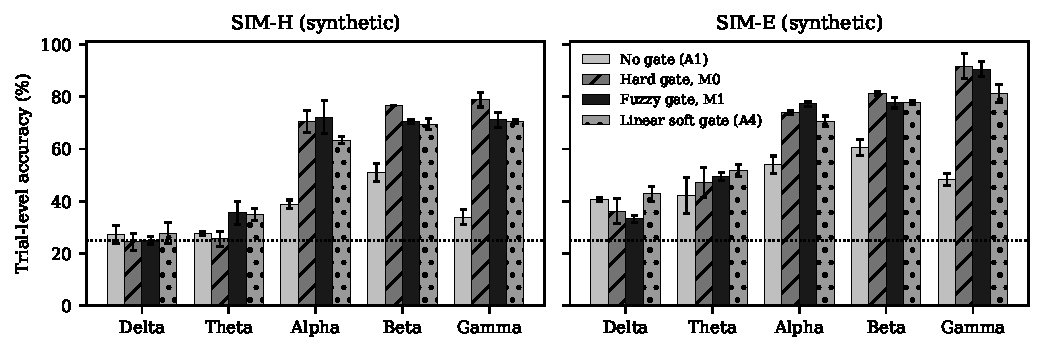
\includegraphics[width=\linewidth]{generated/fig_bands.pdf}
\caption{Trial-level accuracy per band, G-pupil, protocol P1\simnote{} (mean $\pm$ SD over 3 seeds). The dotted line marks chance (25\%).}
\label{fig:bands}
\end{figure}

\subsection{Class-wise behaviour}
Figure~\ref{fig:cm} shows the confusion matrices of M0 and M1 for the best band of SIM-E (gamma, P1, pooled over three seeds, 45 trials per class). The two gates make almost the same errors. Sad, happy and neutral trials are recognised almost perfectly, and fear is the weak class: 31 of 45 fear trials are correct under M0 and 29 under M1, with most errors assigned to neutral (12 and 13 trials). This is consistent with the generator, in which the bursty broadband fear component is the least stationary within a window.

\begin{figure}[t]
\centering
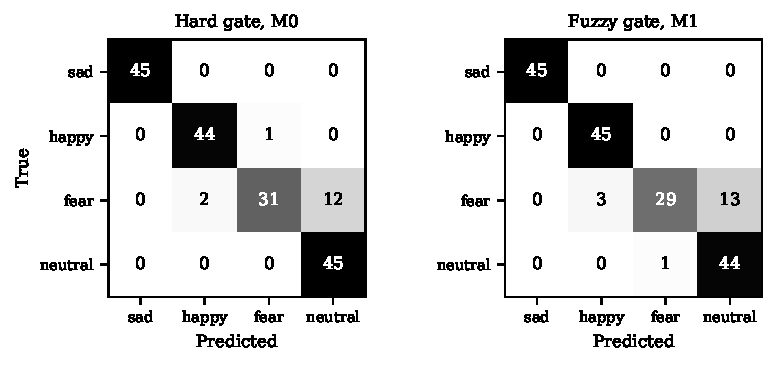
\includegraphics[width=0.72\linewidth]{generated/fig_confusion.pdf}
\caption{Trial-level confusion matrices for M0 and M1, SIM-E, gamma band, G-pupil, P1, pooled over three seeds\simnote.}
\label{fig:cm}
\end{figure}

\subsection{Statistical comparison}
Table~\ref{tab:stats} reports the paired tests. With G-pupil, M1 differed from M0 by a median of 0 to $-1.7$~pp, and no difference approached significance ($p=0.407$--$0.916$). M1 did not differ significantly from the linear gate either ($p\geq0.093$). M1 was, however, clearly better than no gating ($p\leq0.005$; 11--15 wins out of 15 pairs; median gains 16.7--21.7~pp). The exact McNemar tests for the best bands agree: on SIM-H alpha, 30 trials were correct only under M1 and 27 only under M0 ($p=0.79$); on SIM-E gamma the counts were 12 and 14 ($p=0.85$). With G-mRMR, two of the twelve M1 comparisons reached $p<0.05$ (M1 vs M0, LOSO, SIM-E, median $+1.7$~pp, $p=0.049$; and M1 vs A1 in the same cell, $p=0.041$). Given the number of tests performed, these isolated results do not survive correction for multiple comparisons and are not taken as evidence of an advantage.

\begin{table}[t]
\centering\scriptsize
\caption{Paired Wilcoxon signed-rank tests of M1 against other gates over 15 (seed, band) pairs\simnote. $\Delta$acc: M1 minus comparator. Uncorrected $p$-values}\label{tab:stats}
\resizebox{\linewidth}{!}{\begin{tabular}{@{}lllcccc@{}}
\toprule
Gate feature & Protocol & Data & Comparison & Median $\Delta$acc (pp) & W / wins--ties--losses & $p$\\
\midrule
pupil-Y & trial-disjoint 5-fold & SIM-H & M1 vs Hard gate & +0.0 & 41 / 6--2--7 & 0.752\\
pupil-Y & trial-disjoint 5-fold & SIM-H & M1 vs Linear soft gate & +0.0 & 34 / 7--2--6 & 0.442\\
pupil-Y & trial-disjoint 5-fold & SIM-H & M1 vs No gate & +18.3 & 4 / 13--1--1 & 0.002\\
pupil-Y & trial-disjoint 5-fold & SIM-E & M1 vs Hard gate & -1.7 & 58 / 7--0--8 & 0.886\\
pupil-Y & trial-disjoint 5-fold & SIM-E & M1 vs Linear soft gate & +0.0 & 44 / 7--1--7 & 0.572\\
pupil-Y & trial-disjoint 5-fold & SIM-E & M1 vs No gate & +20.0 & 10 / 11--0--4 & 0.005\\
\midrule
pupil-Y & LOSO & SIM-H & M1 vs Hard gate & +0.0 & 16 / 5--6--4 & 0.407\\
pupil-Y & LOSO & SIM-H & M1 vs Linear soft gate & -1.7 & 30 / 5--0--10 & 0.093\\
pupil-Y & LOSO & SIM-H & M1 vs No gate & +16.7 & 0 / 14--1--0 & 0.001\\
pupil-Y & LOSO & SIM-E & M1 vs Hard gate & +0.0 & 44 / 7--2--6 & 0.916\\
pupil-Y & LOSO & SIM-E & M1 vs Linear soft gate & +1.7 & 31 / 8--2--5 & 0.308\\
pupil-Y & LOSO & SIM-E & M1 vs No gate & +21.7 & 0 / 15--0--0 & 0.001\\
\midrule
mRMR & trial-disjoint 5-fold & SIM-H & M1 vs Hard gate & +0.0 & 45 / 7--2--6 & 0.972\\
mRMR & trial-disjoint 5-fold & SIM-H & M1 vs Linear soft gate & +0.0 & 49 / 7--1--7 & 0.826\\
mRMR & trial-disjoint 5-fold & SIM-H & M1 vs No gate & +1.7 & 50 / 8--0--7 & 0.585\\
mRMR & trial-disjoint 5-fold & SIM-E & M1 vs Hard gate & +3.3 & 27 / 9--1--5 & 0.109\\
mRMR & trial-disjoint 5-fold & SIM-E & M1 vs Linear soft gate & +0.0 & 32 / 5--4--6 & 0.929\\
mRMR & trial-disjoint 5-fold & SIM-E & M1 vs No gate & +1.7 & 53 / 8--0--7 & 0.691\\
\midrule
mRMR & LOSO & SIM-H & M1 vs Hard gate & +1.7 & 37 / 8--1--6 & 0.328\\
mRMR & LOSO & SIM-H & M1 vs Linear soft gate & +0.0 & 18 / 4--4--7 & 0.180\\
mRMR & LOSO & SIM-H & M1 vs No gate & -1.7 & 24 / 4--2--9 & 0.140\\
mRMR & LOSO & SIM-E & M1 vs Hard gate & +1.7 & 26 / 10--0--5 & 0.049\\
mRMR & LOSO & SIM-E & M1 vs Linear soft gate & +1.7 & 28 / 9--1--5 & 0.130\\
mRMR & LOSO & SIM-E & M1 vs No gate & +8.3 & 24 / 11--0--4 & 0.041\\
\bottomrule
\end{tabular}
}
\end{table}

\subsection{Robustness to gate-signal noise}
The main argument for fuzzy gating is tolerance of an uncertain eye signal. Table~\ref{tab:noise} and Fig.~\ref{fig:noise} test this directly. As noise increased from $\kappa=0$ to $\kappa=2$, the AUC of the pupil feature for detecting episodes fell from about 0.99 to 0.72--0.73, and all gated configurations lost accuracy (M0: 55.2\% to 43.8\% on SIM-H and 66.0\% to 55.1\% on SIM-E). The fuzzy gate did \emph{not} degrade more gracefully. Its mean deficit relative to M0 was between $-1.1$ and $-3.4$~pp at every non-zero noise level, although none of these differences was significant ($p\geq0.19$). At every noise level all gates remained above the no-gate reference. The hypothesis that fuzzy gating confers robustness to gate noise is therefore not supported by this simulation.

\begin{table}[t]
\centering\scriptsize
\caption{Mean trial accuracy (\%) under gate-signal noise\simnote{} (G-pupil, P1, mean over 5 bands $\times$ 3 seeds). Gate AUC: episode-detection AUC of the noisy pupil feature. $p$: Wilcoxon, M1 vs M0}\label{tab:noise}
\begin{tabular}{@{}lcccccccc@{}}
\toprule
Data & Noise $\kappa$ & Gate AUC & No gate & M0 hard & M1 fuzzy & A4 linear & $\Delta$(M1$-$M0) & $p$\\
\midrule
SIM-H & 0 & 0.987 & 35.8 & 55.2 & 54.9 & 53.2 & -0.3 & 0.752\\
 & 0.5 & 0.943 & 35.8 & 53.1 & 51.7 & 52.0 & -1.4 & 0.299\\
 & 1 & 0.852 & 35.8 & 50.0 & 47.4 & 47.4 & -2.6 & 0.191\\
 & 2 & 0.721 & 35.8 & 43.8 & 41.7 & 44.3 & -2.1 & 0.310\\
\midrule
SIM-E & 0 & 0.985 & 49.1 & 66.0 & 65.7 & 64.8 & -0.3 & 0.886\\
 & 0.5 & 0.943 & 49.1 & 65.0 & 63.9 & 61.7 & -1.1 & 0.506\\
 & 1 & 0.855 & 49.1 & 62.7 & 59.8 & 60.4 & -2.9 & 0.258\\
 & 2 & 0.729 & 49.1 & 55.1 & 51.7 & 53.8 & -3.4 & 0.363\\
\bottomrule
\end{tabular}

\end{table}

\begin{figure}[t]
\centering
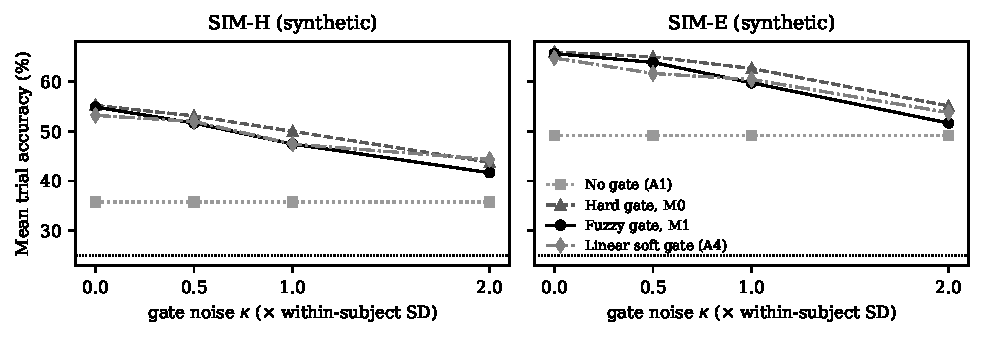
\includegraphics[width=0.95\linewidth]{generated/fig_noise.pdf}
\caption{Mean trial accuracy as a function of gate-signal noise $\kappa$, G-pupil, P1\simnote.}
\label{fig:noise}
\end{figure}

\subsection{Computational cost}
Table~\ref{tab:cost} reports the effective share of training windows (sum of weights divided by the number of windows) and the mean wall-clock time per band and run (all folds). Because the GA dominates the run time and stops adaptively, all gates cost about the same, 10.9--11.6~s per band. The baseline's argument that gating saves computation by discarding windows \cite{FarhadiSedehi2024a} applies to feature extraction on real-time hardware, which is identical here because entropies were precomputed for all windows. In such a setting the fuzzy gate would forgo that saving, since every window must be processed.

\begin{table}[t]
\centering\small
\caption{Computational cost\simnote{} (mean over all runs)}\label{tab:cost}
\begin{tabular}{@{}lcc@{}}
\toprule
Configuration & Effective training windows (\%) & Time per band, all folds (s)\\
\midrule
No gate (A1) & 100.0 & 11.6\\
Hard gate, M0 & 41.8 & 11.0\\
Fuzzy gate, M1 & 45.7 & 11.2\\
Linear soft gate (A4) & 44.3 & 10.9\\
\bottomrule
\end{tabular}

\end{table}

\subsection{Relation to the team's earlier window-level runs}
Before this study, the baseline pipeline (M0 only) had been run on the same synthetic datasets with the original protocol, in which 4-s windows are pooled and randomly split into five folds and accuracy is measured per window. Those runs are reported in Table~\ref{tab:prev} for completeness. They are window-level accuracies on the retained windows, not trial-level accuracies, and are therefore not directly comparable with Tables~\ref{tab:main}--\ref{tab:noise}. Two observations agree with the present study: the run that used the fixation-duration gate selected by mRMR reached at most 47.8\% (SIM-H) and 56.7\% (SIM-E), whereas the run with the pupil gate reached 75.0--75.8\% in beta and gamma on SIM-E. On these synthetic data, where windows are generated independently given the episode mask, the trial-grouped protocol gave values similar to the pooled protocol (e.g.\ SIM-H beta 45.8\% vs 47.8\%). This similarity is not expected to hold for real EEG, where neighbouring windows are strongly correlated \cite{Li2021}.

\begin{table}[t]
\centering\scriptsize
\caption{Earlier baseline (M0) runs on the synthetic data with the original window-level protocol\simnote{} (window accuracy on retained windows, \%, mean $\pm$ SD over 5 folds, 3 fuzzy levels)}\label{tab:prev}
\resizebox{\linewidth}{!}{\begin{tabular}{@{}llccccc@{}}
\toprule
Run & Gate feature / protocol & Delta & Theta & Alpha & Beta & Gamma\\
\midrule
SIM-H & mRMR (\texttt{fix\_dur\_mean}) / window 5-fold & 20.8 $\pm$ 2.3 & 23.6 $\pm$ 4.2 & 43.3 $\pm$ 2.7 & 47.8 $\pm$ 4.8 & 47.2 $\pm$ 3.4\\
SIM-H & mRMR (\texttt{fix\_dur\_mean}) / trial-grouped & 26.1 $\pm$ 4.2 & 25.0 $\pm$ 2.8 & 42.5 $\pm$ 4.8 & 45.8 $\pm$ 7.1 & 46.7 $\pm$ 3.4\\
SIM-E & mRMR (\texttt{fix\_dur\_mean}) / window 5-fold & 24.2 $\pm$ 5.1 & 30.8 $\pm$ 5.9 & 50.8 $\pm$ 2.6 & 56.7 $\pm$ 3.2 & 54.2 $\pm$ 4.7\\
SIM-E & \texttt{pupil\_y\_mean} / window 5-fold & 33.6 $\pm$ 4.4 & 35.3 $\pm$ 5.9 & 59.7 $\pm$ 3.2 & 75.0 $\pm$ 6.8 & 75.8 $\pm$ 2.4\\
\bottomrule
\end{tabular}
}
\end{table}

\subsection{Discussion}
Three findings stand out. First, \emph{the gating signal matters far more than the gating function}. With a signal that tracks the informative windows, any of the three gates raised mean accuracy by 13--19~pp over no gating; with a class-discriminative but episode-blind signal, none helped reliably. This exposes a weakness of the original procedure, which selects the gate feature by its mutual information with the class label. Such a criterion rewards features that differ \emph{between} classes, whereas a gate needs a feature that differs \emph{within} a trial between affective and non-affective moments. In our simulation the two criteria point to different features. In real data, label-driven selection can also pick up session or stimulus confounds.

Second, \emph{fuzzy and hard gating were statistically indistinguishable}, and the fuzzy gate was not better than a plain linear soft gate. With one input and a Ruspini partition, the fuzzy gate is a piecewise-linear soft threshold, so this equivalence is unsurprising in hindsight. The data show no benefit from the fuzzy formulation itself beyond what its softness provides.

Third, \emph{softness did not buy robustness}. The fuzzy gate keeps every window with weight at least $r_L$ and gives Medium-range windows substantial weight, which lowers its weighted precision (79\% vs 90--93\% for the hard gate). When class information is confined to the episodes, as in this simulation, the extra non-episode mass dilutes the training data and the trial vote. When gate noise rises, the soft gate does not recover this loss. A softer gate would be expected to help mainly when the gating signal is weakly informative and the hard gate's ranking within a trial becomes unreliable. Even at $\kappa=2$ (AUC 0.72), that point had not been reached. The design parameters ($r_L=0.1$, the width of the Medium set) were fixed a priori, and a sharper partition or a learned partition might change this balance. That is a question for future work, not a finding of this study.

The interpretability argument for fuzzy gating is unaffected by these results. The gate can be stated as three linguistic rules, and a reviewer can read off how much each window contributed. The value of that transparency has to be weighed against the absence of an accuracy advantage.

% =====================================================================
\section{Limitations}
\label{sec:limits}
(i) \emph{All results are on synthetic data.} The generator encodes the assumptions that motivate gating, namely intermittent affective information and pupil dilation co-occurring with it. The results show how the gates behave if these assumptions hold, not whether they hold in real recordings or what accuracy would be obtained on real EEG. (ii) The synthetic data are small (5 subjects, 60 trials), so differences of a few percentage points cannot be resolved. With 15 paired observations per test, the study can detect only moderate effects. (iii) Synthetic windows are conditionally independent given the episode mask, so the leakage that pooled window-level cross-validation causes on real EEG is not reproduced. (iv) The hard-gate threshold rule (within-trial 60th percentile) is our operationalisation of an under-specified description \cite{FarhadiSedehi2024a}, and the fuzzy-gate parameters were not tuned. Other choices could shift the comparison. (v) The pupil signal in the simulation contains no luminance or gaze-position confounds \cite{Mathot2018,Raiturkar2016}, which are major sources of uncertainty in real recordings. (vi) The S-FIS uses only three EEG inputs per band, as in the original method.

% =====================================================================
\section{Conclusion and future work}
\label{sec:conclusion}
This paper compared hard and fuzzy eye-tracking gating of EEG windows within a Sugeno fuzzy rule-mining emotion recognizer. All other components were held fixed, and the evaluation was a controlled simulation in which the affectively relevant windows are known. The fuzzy gate maps Low/Medium/High memberships of the normalised eye-tracking feature to continuous window weights that enter feature selection, rule mining, GA fitness and trial-level aggregation, and it contains the hard gate as a limiting case. On two synthetic datasets, under trial- and subject-disjoint cross-validation, gating with an informative pupil signal improved trial accuracy over no gating by median paired gains of 16.7--21.7 percentage points. Fuzzy and hard gating, however, were statistically indistinguishable. The fuzzy gate was not better than a linear soft gate and not more robust to gate-signal noise. Selecting the gate feature by its relevance to the class label, as in the original method, chose fixation features that did not locate the informative windows. In this setting, how well the gating signal identifies the relevant windows matters far more than the form of the gate.

Future work will (1) evaluate the gates on real simultaneous EEG and eye-tracking recordings such as SEED-IV \cite{Zheng2019}, MAHNOB-HCI \cite{Soleymani2012db} or ZuCo \cite{Hollenstein2018}, under subject-disjoint protocols; (2) select gating features by within-trial relevance criteria rather than class relevance; (3) correct pupil signals for luminance before gating \cite{Raiturkar2016}; (4) study multi-input fuzzy gates and gate parameters learned under nested cross-validation \cite{Jang1993}; and (5) extend the simulation with temporally correlated windows and realistic ocular confounds.

% =====================================================================
\section*{Declarations}
\noindent\textbf{Funding} \pending{to be completed by the authors}\\
\textbf{Conflict of interest} \pending{to be completed by the authors}\\
\textbf{Data availability} No real human data were used. The synthetic datasets can be regenerated exactly with \texttt{python -m gfer.demo --out data/demo --seed 0} (SIM-H) and \texttt{python -m gfer.demo --out data/demo\_easy --seed 1 --signal-strength 3} (SIM-E).\\
\textbf{Code availability} All code, raw results and the scripts that generate every table and figure (\texttt{gfer/compare.py}, \texttt{gfer/analyze\_sim.py}, \texttt{gfer/analyze\_noise.py}) are available at \pending{repository URL}.\\
\textbf{Author contributions} \pending{to be completed by the authors}

% =====================================================================
\small
